\cleardoublepage

\chapter{Imprimerie Nationale}

%%%%%%%%%%%%%%%%%%%%%%%%%%%%%%%%%%%%%%%%%%%%%%%%%%%%%%%%%%%%%%%%%%%%%%%%%%%
%%%%%%%%%%%%%%%%%%%%%%%%%%%%%%%%%%%%%%%%%%%%%%%%%%%%%%%%%%%%%%%%%%%%%%%%%%%
%%%%%%%%%%%%%%%%%%%%%%%%%%%%%%%%%%%%%%%%%%%%%%%%%%%%%%%%%%%%%%%%%%%%%%%%%%%
%%%%%%%%%%%%%%%%%%%%%%%%%%%%%%%%%%%%%%%%%%%%%%%%%%%%%%%%%%%%%%%%%%%%%%%%%%%
%%%%%%%%%%%%%%%%%%%%%%%%%%%%%%%%%%%%%%%%%%%%%%%%%%%%%%%%%%%%%%%%%%%%%%%%%%%

\section{L'administration}

L'application est divisée en divers niveaux afin d'apporter une gestion fine.
La figure \ref{niveaux_administration} représente les différents niveaux présentés dans cette section.
\begin{figure}[!h]
	\center
	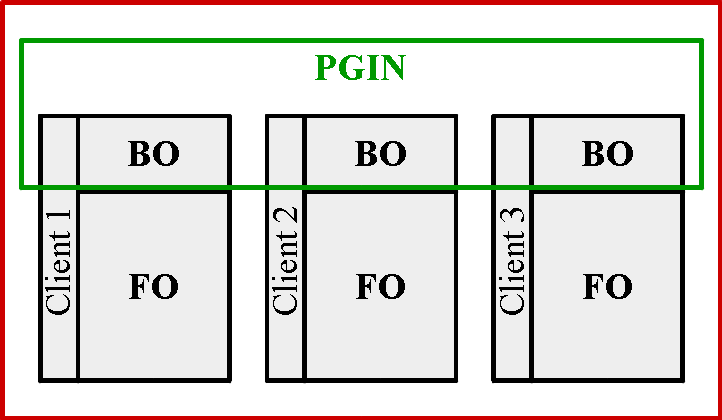
\includegraphics[width=0.8\textwidth]{img/niveaux_administration.png}
	\caption{Niveaux d'administration de l'application}
	\label{niveaux_administration}
\end{figure}

%%%%%%%%%%%%%%%%%%%%%%%%%%%%%%%%%%%%%%%%%%%%%%%%%%%%%%%%%%%%%%%%%%%%%%%%%%%
%%%%%%%%%%%%%%%%%%%%%%%%%%%%%%%%%%%%%%%%%%%%%%%%%%%%%%%%%%%%%%%%%%%%%%%%%%%
%%%%%%%%%%%%%%%%%%%%%%%%%%%%%%%%%%%%%%%%%%%%%%%%%%%%%%%%%%%%%%%%%%%%%%%%%%%

\subsection{Le Front Office}

Le \textit{Front Office} (FO) est la partie accessible par les utilisateurs finaux.
Elle propose les principales fonctionnalités principales de l'application.
Dans notre cas il s'agit des fonctions de gestion des supports : demande, validation, révocation, \ldots

%%%%%%%%%%%%%%%%%%%%%%%%%%%%%%%%%%%%%%%%%%%%%%%%%%%%%%%%%%%%%%%%%%%%%%%%%%%
%%%%%%%%%%%%%%%%%%%%%%%%%%%%%%%%%%%%%%%%%%%%%%%%%%%%%%%%%%%%%%%%%%%%%%%%%%%
%%%%%%%%%%%%%%%%%%%%%%%%%%%%%%%%%%%%%%%%%%%%%%%%%%%%%%%%%%%%%%%%%%%%%%%%%%%

\subsection{Le Back Office}

Le \textit{Back Office} (BO) est quant à lui destinée aux administrateurs de l'application.
L'objectif de cette partie est de gérer les utilisateurs et droits, mais aussi de gérer les données "statiques" qui apparaitront dans la partie front office comme par exemple l'ensemble des supports disponibles.

Il s'agit du niveau sur lequel j'ai travaillé durant mon stage et que je vous présenterai dans ce chapitre.
\\

L'imprimerie nationale souhaite proposer cette application à divers clients.
L'architecture sera donc \textit{multi-tenant}, c'est-à-dire que chaque client possèdera son propre utilisateur et ses problèmes tables dans la base de données.

%%%%%%%%%%%%%%%%%%%%%%%%%%%%%%%%%%%%%%%%%%%%%%%%%%%%%%%%%%%%%%%%%%%%%%%%%%%

\subsubsection{Administration}

Il est nécessaire que chaque client puisse administrer ses proposer données qui lui sont propre, sans impacter les données des autres clients.
Pour cela un niveau "Administrateur" a été mis en place.

%%%%%%%%%%%%%%%%%%%%%%%%%%%%%%%%%%%%%%%%%%%%%%%%%%%%%%%%%%%%%%%%%%%%%%%%%%%

\subsubsection{PGIN}

L'imprimerie va produire des cartes pour l'ensemble de ses clients.
Ainsi des données seront communes à chacune des clients et il est nécessaire de pouvoir les gérer efficacement.
De plus, il est nécessaire de pouvoir administrer l'application de chacun des clients, en cas de problème ou pour effectuer des maintenances.

Dans cet objectif, un niveau "PGIN" (signifiant TODO PG Imprimerie Nationale) a été mis en place afin d'administrer l'ensemble des données des clients.

%%%%%%%%%%%%%%%%%%%%%%%%%%%%%%%%%%%%%%%%%%%%%%%%%%%%%%%%%%%%%%%%%%%%%%%%%%%
%%%%%%%%%%%%%%%%%%%%%%%%%%%%%%%%%%%%%%%%%%%%%%%%%%%%%%%%%%%%%%%%%%%%%%%%%%%
%%%%%%%%%%%%%%%%%%%%%%%%%%%%%%%%%%%%%%%%%%%%%%%%%%%%%%%%%%%%%%%%%%%%%%%%%%%
%%%%%%%%%%%%%%%%%%%%%%%%%%%%%%%%%%%%%%%%%%%%%%%%%%%%%%%%%%%%%%%%%%%%%%%%%%%
%%%%%%%%%%%%%%%%%%%%%%%%%%%%%%%%%%%%%%%%%%%%%%%%%%%%%%%%%%%%%%%%%%%%%%%%%%%

\section{Gestion des instances}

%%%%%%%%%%%%%%%%%%%%%%%%%%%%%%%%%%%%%%%%%%%%%%%%%%%%%%%%%%%%%%%%%%%%%%%%%%%
%%%%%%%%%%%%%%%%%%%%%%%%%%%%%%%%%%%%%%%%%%%%%%%%%%%%%%%%%%%%%%%%%%%%%%%%%%%
%%%%%%%%%%%%%%%%%%%%%%%%%%%%%%%%%%%%%%%%%%%%%%%%%%%%%%%%%%%%%%%%%%%%%%%%%%%

\subsection{Présentation}

Une instance, aussi appelé niveau hiérarchique, et une entité de l'entreprise.
Les différentes instances forment une hiérarchie, représentée sous la forme d'un arbre.
L'instance racine est la compagnie et est unique pour un client donné.
Les instances sous-jacentes sont les divisions, et les feuilles sont les domaines.
La solution actuelle se limite à trois niveaux dans la hiérarchie.

À titre d'exemple, on peut représenter Sopra Group France qui est composée de divisions (Rhône-Alpes Auvergne, \ldots) qui sont elles-même composées d'agences (Clermont Ferrand, Lyon, \ldots).
La figure \ref{hierarchie_Sopra_Group} représente la hiérarchie de Sopra Group France.
\begin{figure}[!h]
	\center
	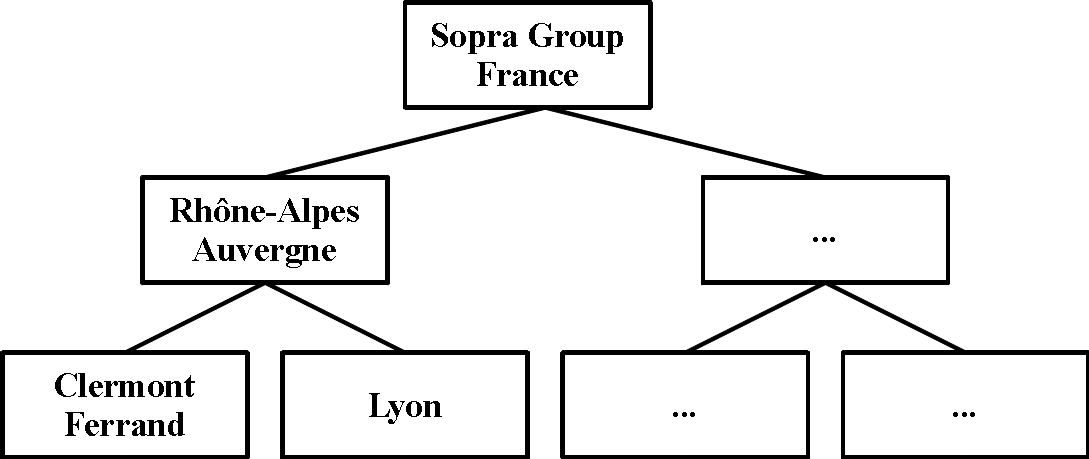
\includegraphics[width=0.8\textwidth]{img/hierarchie_Sopra_Group.png}
	\caption{Hiérarchie de Sopra Group France}
	\label{hierarchie_Sopra_Group}
\end{figure}
~~\\

%%%%%%%%%%%%%%%%%%%%%%%%%%%%%%%%%%%%%%%%%%%%%%%%%%%%%%%%%%%%%%%%%%%%%%%%%%%
%%%%%%%%%%%%%%%%%%%%%%%%%%%%%%%%%%%%%%%%%%%%%%%%%%%%%%%%%%%%%%%%%%%%%%%%%%%
%%%%%%%%%%%%%%%%%%%%%%%%%%%%%%%%%%%%%%%%%%%%%%%%%%%%%%%%%%%%%%%%%%%%%%%%%%%

\subsection{Les écrans}

J'ai tout d'abord travaillé sur la gestion des instances.
L'objectif est de pouvoir effectuer les opérations courantes (affichage, modification, création, suppression), ainsi que l'association des utilisateurs.
La figure \ref{instances_UML} est le diagramme UML des instances.
\begin{figure}[!h]
	\center
	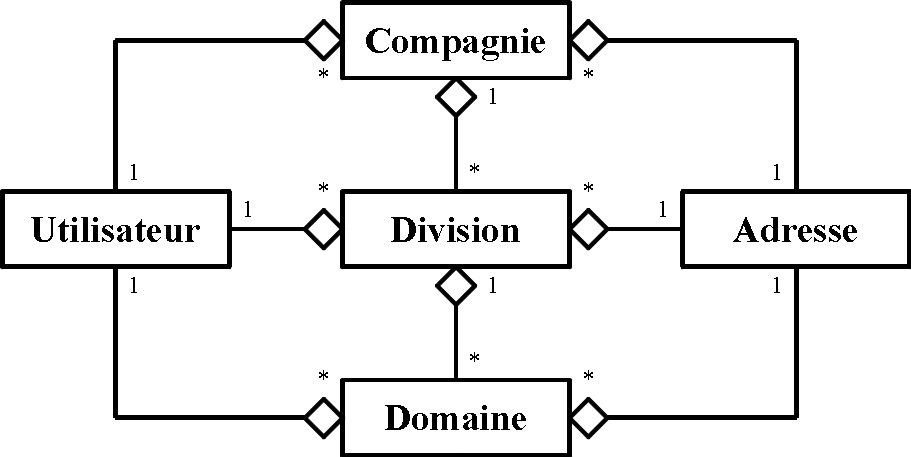
\includegraphics[width=0.8\textwidth]{img/instances_UML.png}
	\caption{Diagramme UML des instances}
	\label{instances_UML}
\end{figure}

%%%%%%%%%%%%%%%%%%%%%%%%%%%%%%%%%%%%%%%%%%%%%%%%%%%%%%%%%%%%%%%%%%%%%%%%%%%

\subsubsection{Managing}

L'écran d'accueil de la gestion affiche la hiérarchie des instances, présenté sur la figure \ref{instances_managing} qui en est une capture d'écran.
Des boutons d'action permettent d'agir sur l'instance sélectionnée.
\begin{figure}[!h]
	\center
	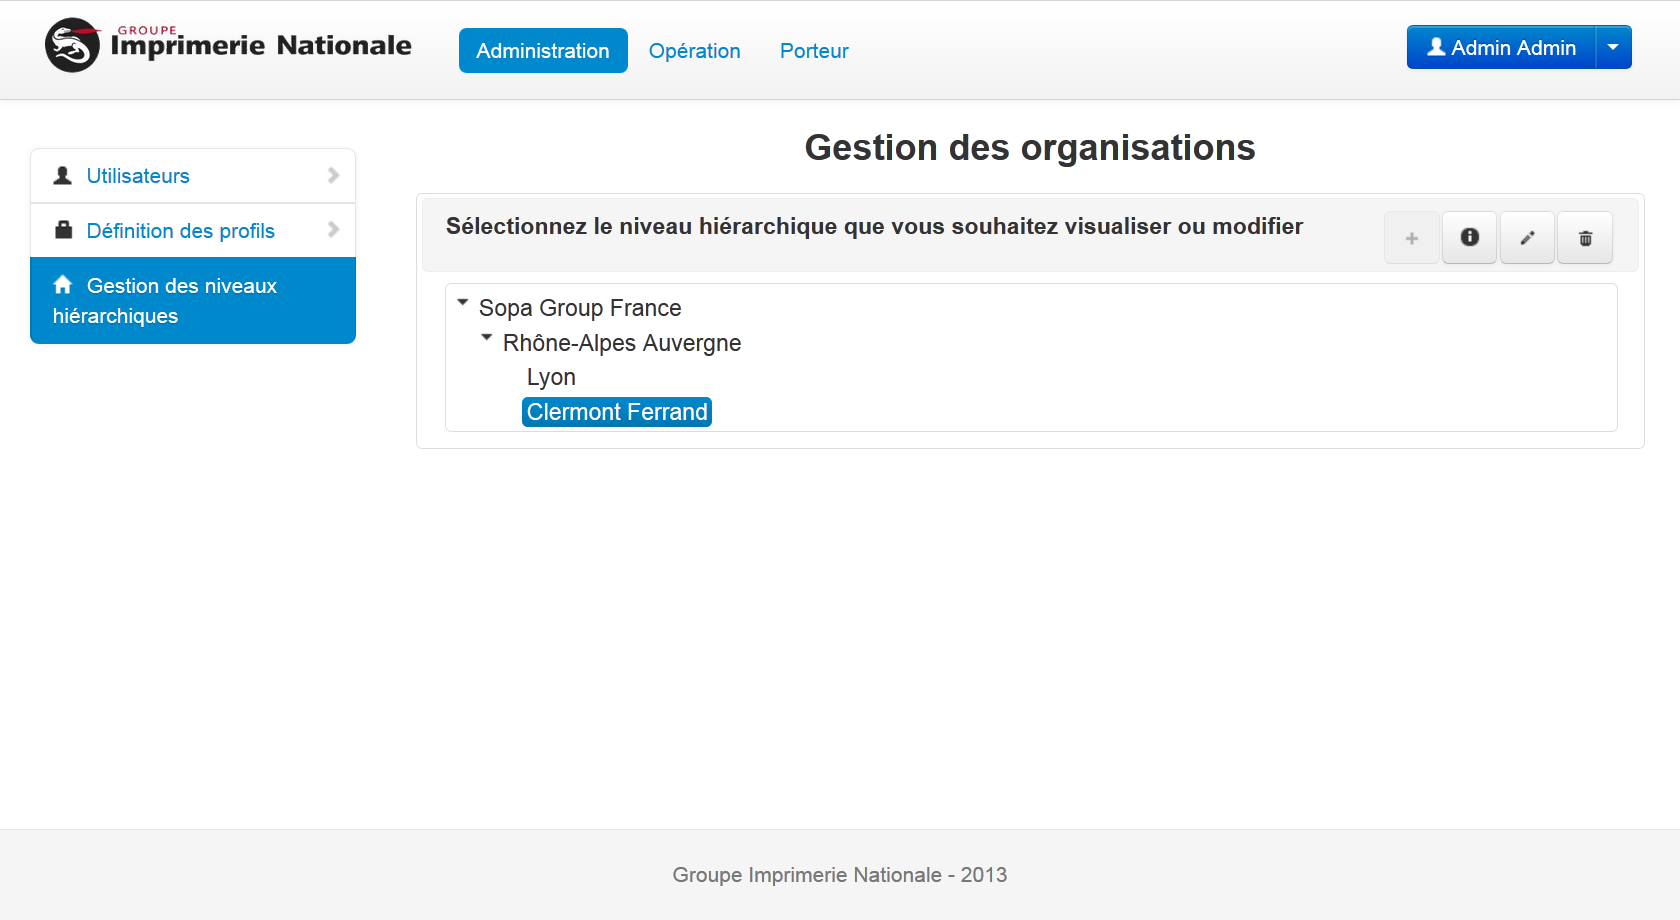
\includegraphics[width=0.8\textwidth]{img/instances_managing.png}
	\caption{Managing des instances}
	\label{instances_managing}
\end{figure}
~~\\

La suppression d'une instance se fait simplement en sélectionnant une instance dans la hiérarchie de l'écran puis en cliquant sur le bouton "Supprimer".
Pour des raisons de sécurité, il est impossible de supprimer une instance si celle-ci possède des liens avec d'autres données dans la base de données.
Par exemple il est impossible de supprimer une division s'il existe des domaines sous-jacents.

%%%%%%%%%%%%%%%%%%%%%%%%%%%%%%%%%%%%%%%%%%%%%%%%%%%%%%%%%%%%%%%%%%%%%%%%%%%

\subsubsection{Affichage, modification et création}

Dans ce type d'actions, il existe deux types d'écran.
L'affichage affiche simplement les valeurs des différents champs.
Les écrans de création et modification affichent quand à eux une zone de saisie, où les champs sont pré-remplies par la valeur dans le cas d'une modification.

Dans les trois cas il est possible d'afficher les informations des instances parentes en cliquant sur l'onglet correspondant.
Par exemple lorsque l'on modifie une division, la division et la compagnie sont affichées (sans modification possible).
Cela permet à l'utilisateur de connaître quelle instance il manipule et où elle se situe dans la hiérarchie.
La figure \ref{instances_modification} est une capture d'écran de la fenêtre de modification d'une division.
\begin{figure}[!h]
	\center
	
\includegraphics[width=0.4\textwidth]{img/instances_modification.png}
	\caption{Modification d'un domaine}
	\label{instances_modification}
\end{figure}

%%%%%%%%%%%%%%%%%%%%%%%%%%%%%%%%%%%%%%%%%%%%%%%%%%%%%%%%%%%%%%%%%%%%%%%%%%%

\subsubsection{Les utilisateurs}

Chaque utilisateur de l'application est rattaché à une instance.
La modification d'une instance permet aussi d'associer de nouveaux utilisateurs ou de supprimer des nouveaux utilisateurs à l'instance.

La figure \ref{instances_utilisateurs} est l'écran d'affectation, composé de deux parties : la liste des utilisateurs disponibles avec un filtre de recherche, et la liste des utilisateurs associés.
Les deux listes sont complémentaires, c'est-à-dire que l'association d'un utilisateur à l'instance le fera passer de la liste des disponibles à la liste des associés.
L'association se fait en sélectionnant des utilisateurs dans une des liste puis en cliquant sur le bouton "flèche du haut" ou "flèche du bas" pour ajouter ou retirer des utilisateurs.
\begin{figure}[!h]
	\center
	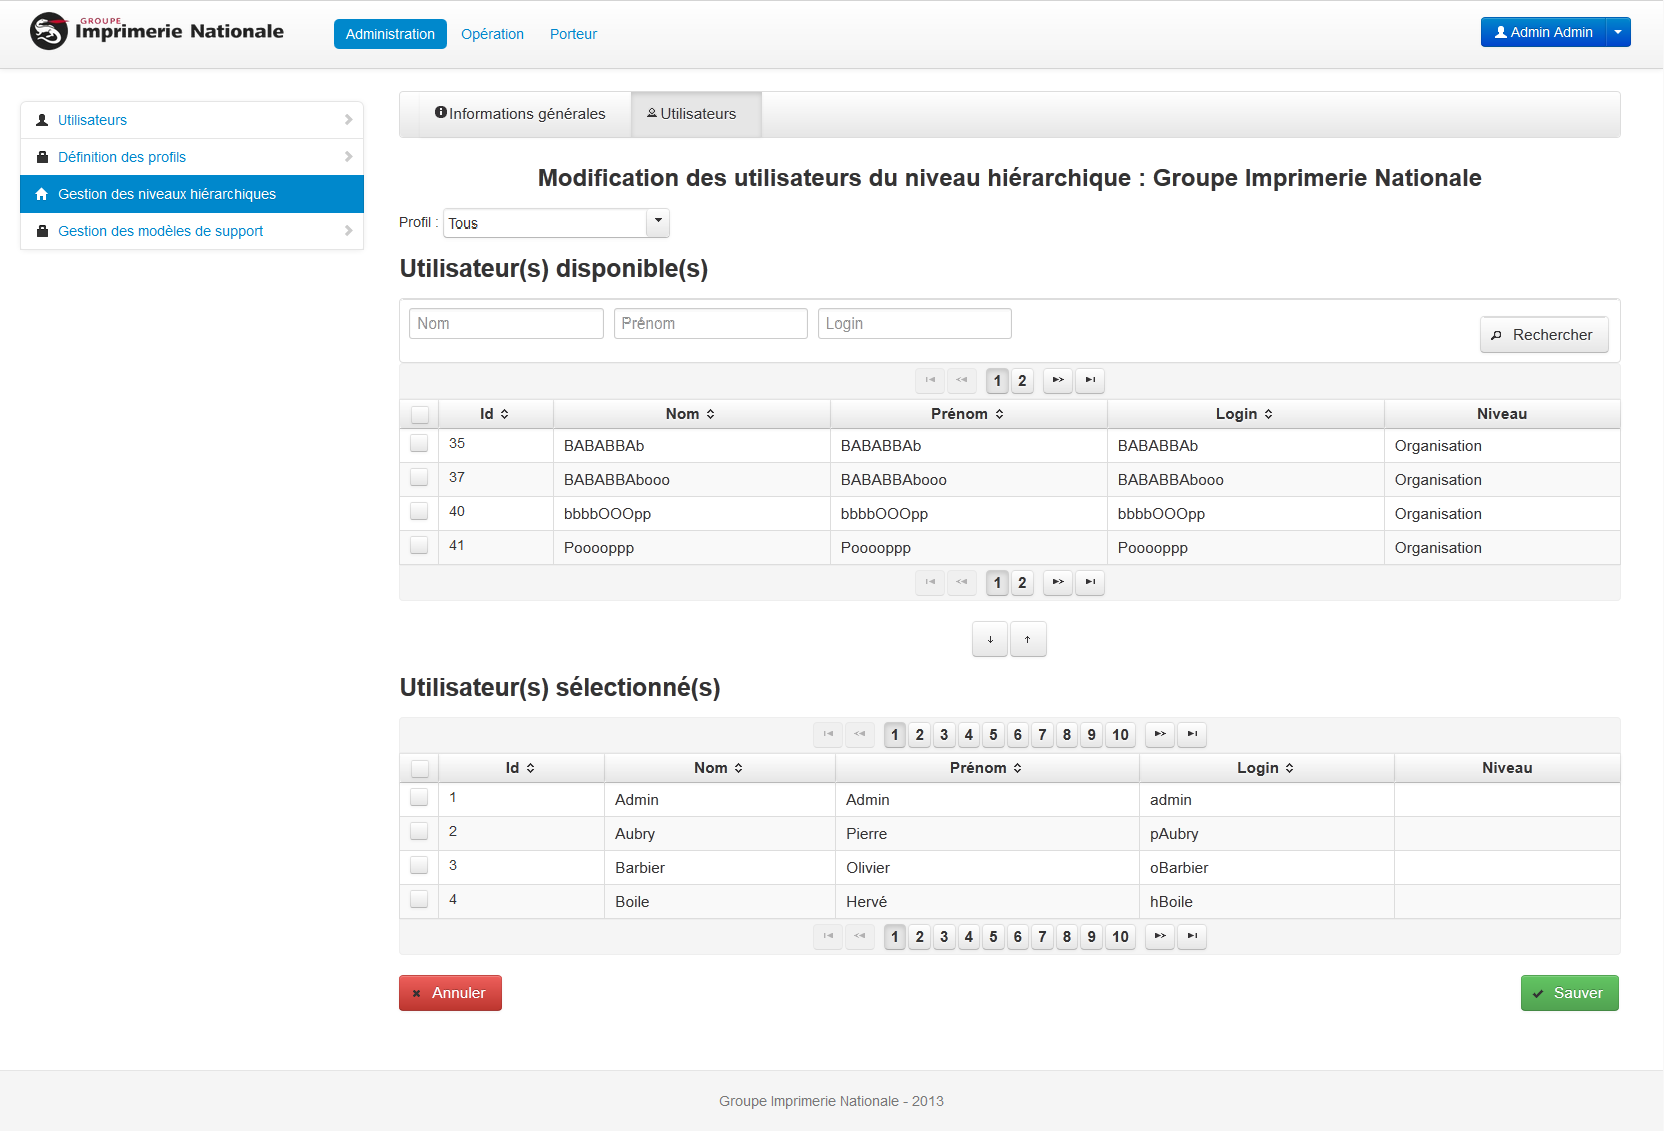
\includegraphics[width=0.4\textwidth]{img/instances_utilisateurs.png}
	\caption{Association d'utilisateurs à une instance}
	\label{instances_utilisateurs}
\end{figure}

%%%%%%%%%%%%%%%%%%%%%%%%%%%%%%%%%%%%%%%%%%%%%%%%%%%%%%%%%%%%%%%%%%%%%%%%%%%
%%%%%%%%%%%%%%%%%%%%%%%%%%%%%%%%%%%%%%%%%%%%%%%%%%%%%%%%%%%%%%%%%%%%%%%%%%%
%%%%%%%%%%%%%%%%%%%%%%%%%%%%%%%%%%%%%%%%%%%%%%%%%%%%%%%%%%%%%%%%%%%%%%%%%%%
%%%%%%%%%%%%%%%%%%%%%%%%%%%%%%%%%%%%%%%%%%%%%%%%%%%%%%%%%%%%%%%%%%%%%%%%%%%
%%%%%%%%%%%%%%%%%%%%%%%%%%%%%%%%%%%%%%%%%%%%%%%%%%%%%%%%%%%%%%%%%%%%%%%%%%%

\section{Gestion des profils}

%%%%%%%%%%%%%%%%%%%%%%%%%%%%%%%%%%%%%%%%%%%%%%%%%%%%%%%%%%%%%%%%%%%%%%%%%%%
%%%%%%%%%%%%%%%%%%%%%%%%%%%%%%%%%%%%%%%%%%%%%%%%%%%%%%%%%%%%%%%%%%%%%%%%%%%
%%%%%%%%%%%%%%%%%%%%%%%%%%%%%%%%%%%%%%%%%%%%%%%%%%%%%%%%%%%%%%%%%%%%%%%%%%%

\subsection{Généralités}

Les différentes restrictions dans l'application sont gérées par des droits.
En fonction des droits que possède l'utilisateur, celui-ci verra des entrées dans les menus, des boutons d'action, \ldots cachés.
Cette gestion des droits se fait finement par l'intermédiaire des profils, comme détaillé dans la section \ref{Gestion des droits}.
\\

L'écran d'affectation des utilisateurs est identique à celui de la figure \ref{instances_utilisateurs}.
L'écran d'affectation des droits diffère uniquement sur les données affichées car ici on y manipule des droits.

%%%%%%%%%%%%%%%%%%%%%%%%%%%%%%%%%%%%%%%%%%%%%%%%%%%%%%%%%%%%%%%%%%%%%%%%%%%
%%%%%%%%%%%%%%%%%%%%%%%%%%%%%%%%%%%%%%%%%%%%%%%%%%%%%%%%%%%%%%%%%%%%%%%%%%%
%%%%%%%%%%%%%%%%%%%%%%%%%%%%%%%%%%%%%%%%%%%%%%%%%%%%%%%%%%%%%%%%%%%%%%%%%%%

\subsection{Différents niveaux}

Il existe deux types de profils : les profils dits spécifiques qui est propre à un client, et les profils dits communs qui sont présent chez l'ensemble des clients.

%%%%%%%%%%%%%%%%%%%%%%%%%%%%%%%%%%%%%%%%%%%%%%%%%%%%%%%%%%%%%%%%%%%%%%%%%%%

\subsubsection{Administration}

Dans le niveau administration, propre à un client, il n'est possible de modifier l'affectation  que l'affectation des utilisateurs aux profils communs.
 

Les profils dits "PGIN" sont ceux

CMS : PGIN ou Commun

%%%%%%%%%%%%%%%%%%%%%%%%%%%%%%%%%%%%%%%%%%%%%%%%%%%%%%%%%%%%%%%%%%%%%%%%%%%

\subsubsection{PGIN}

PGIN : PGIN (Super PGIN ou PGIN) et Commun